

%%%%%%%%%%%%%%%%%%% CS Background
%TM Visual
\begin{frame}{Background -- Computer Science}
 \begin{block}{Turing Machines}
        \begin{figure}
            \centering
            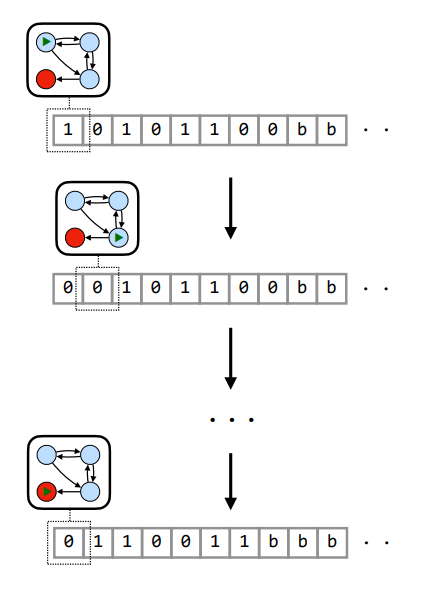
\includegraphics[height=5cm]{TM.png}
            \caption{Graphical representation of a TM}
            \label{fig:TM}
        \end{figure}
    \end{block}
\end{frame}

%Additional Assumptions on TM
\begin{frame}{Background -- Computer Science}
    \begin{block}{Additional Assumptions on TM $M$}
    \begin{enumerate}
        \item $\Sigma = \{0,1,b\}$
        \item If and when $M$ halts on an input, the tape will contain an output string $s\in \{0,1\}^*$ followed by all blank symbols, and the pointer will be set to the start of the tape.
    \end{enumerate}
    Assumptions do not affect the computational capabilities of $M$.
    \end{block}
\end{frame}

% TM as partial functions and UTMs
\begin{frame}{Background -- Computer Science}
    \begin{block}{Turing Machines as Partial Functions}
    Any computation performed by a TM $M$ can be represented as
    \begin{equation*}
        \phi_M:\{0,1\}^* \nrightarrow \{0,1\}^*
    \end{equation*}
    and $\phi_M(x) = y$ indicates that $M$ started with input program $x$ yields the output string $y$.
    \end{block}
    \begin{block}{Universal TM}
    There exist Universal Turing Machines (UTM) such that given a UTM $U$ and any TM $M$, there exists an interpreter program $\sigma_{U,M}$ such that
    \begin{equation*}
        \phi_U(\sigma_{U,M},x) = \phi_M(x)
    \end{equation*}
    \end{block}
\end{frame}

\begin{frame}{Background -- Computer Science}
    \begin{block}{Computability}
    \begin{itemize}
        \item Church Turing Thesis: A function can be calculated by a sequence of formal operations if and only if it is computable by a Turing Machine.
       \item Physical Church Turing Thesis: Any function implemented by a physical process can also be implemented by a Turing Machine
    \end{itemize}
    \end{block}
\end{frame}

%%%%%%%%%%%%%%%%%%%% AIT background 
% Kolomogorov Complexity Defintion
\begin{frame}{Background -- Algorithmic Information Theory}
\begin{block}{Kolmogorov Complexity}
The Kolmogorov complexity $K_U$ of a bitstring $x$ is the length of the shortest input program that when given to a UTM $U$ can produce $x$ as an output:
\begin{equation*}
    K_U(x) :=\min_{z:\phi_U(z) = x}\ell(z)
\end{equation*}
\begin{itemize}
    \item Measure of amount of information in $x$
\end{itemize}
\end{block}
\end{frame}

%Variations on Kolomogorov Complexity
\begin{frame}{Background -- Algorithmic Information Theory}
    \begin{block}{Kolmogorov Complexity of Bitstring $x$}
    \begin{equation*}
        K_U(x) :=\min_{z:\phi_U(z) = x}\ell(z)
    \end{equation*}
    \end{block}
    \begin{block}{Kolmogorov Complexity of a Computable Function $f$}
    \begin{equation*}
        K_U(f) := \min_{M:\phi_M = f} \ell(\sigma_{U,M})
    \end{equation*}
    \end{block}
    \begin{block}{Conditional Kolmogorov Complexity of $x$ Given Bitstring $y$}
\begin{equation*}
    K_U(x|y) = \min_{z:\phi_U(z,y) = x} \ell(z)
\end{equation*}
\end{block}
\end{frame}

%Invariance Theorem
\begin{frame}{Background -- Algorithmic Information Theory}
    \begin{block}{Invariance Theorem}
    For distinct UTM $U$, $U'$:
        \begin{equation*}
            K_{U'}(x) = K_U(x) + O(1)
        \end{equation*}
        Thus, $U$ is usually omitted and we write $K(x)$ for Kolmogorov complexity of $x$
    \end{block}
\end{frame}

%%%%%%%%%%%%% Input Distributions
\begin{frame}{Background -- Input Distributions}
\begin{block}{Coin-Flipping Distribution}
\begin{itemize}
    \item Input string $x$ as random variable with probability distribution $p_X$
    \item Important example: coin flipping distribution of TM $M$
    \begin{equation*}
        m_X^\text{coin}(x) := \begin{cases} 2^{-\ell(x)} &\text{if $x\;\in$ dom $\phi_M$}\\ 0 &\text{otherwise}\end{cases}
    \end{equation*}
    \item With normalizing constant $\Omega_M :=\sum_{x\in\text{ dom }\phi_M} 2^{-\ell(x)}$
    \begin{equation*}
        p_X^\text{coin}(x) = m_X^\text{coin}(x)/\Omega_M
    \end{equation*}
\end{itemize}
\end{block}
\end{frame}


%%%%%%%%%%%% Entropy
%Definition of Entropy
\begin{frame}{Background -- Entropy}
    \begin{block}{Shannon Entropy of Distribution $p_X$}
    \begin{equation*}
    S(p_X) = - \sum_{x\in X} p_X(x)\ln [p_X(x)]    
    \end{equation*}
    \begin{itemize}
        \item Measure of amount of information in $p_X$
        \item $-\ln[p_X(x)]$: ``surprisal", how unexpected, and hence informative, is $x$?
        \item $p_X(x)$: how often do we receive surprise $\ln p_X$
    \end{itemize}
    \end{block}
\end{frame}

%Entropy Production
\begin{frame}{Background -- Entropy}
    \begin{block}{Entropy Production (EP)}
    The expected EP, written $\Sigma (p_X)$ of a physical process with initial state distribution $p_X$ and final state distribution $p_Y$ is:
    \begin{align*}
        \Sigma (p_X) &= S(p_Y) - S(p_X) + \langle Q \rangle_{p_X}/kT
    \end{align*}
    Thermodynamically reversible processes have $\Sigma (p_X)=0$. EP is always nonnegative.
    \end{block}
\end{frame}

